% Beamer Presentation
% LaTeX Template
% Version 1.0 (10/11/12)
%
% This template has been downloaded from:
% http://www.LaTeXTemplates.com
%
% License:
% CC BY-NC-SA 3.0 (http://creativecommons.org/licenses/by-nc-sa/3.0/)
%
%%%%%%%%%%%%%%%%%%%%%%%%%%%%%%%%%%%%%%%%%

%----------------------------------------------------------------------------------------
%	PACKAGES AND THEMES
%----------------------------------------------------------------------------------------


	\documentclass[xcolor=dvipsnames]{beamer}

	\mode<presentation> {

	% The Beamer class comes with a number of default slide themes
	% which change the colors and layouts of slides. Below this is a list
	% of all the themes, uncomment each in turn to see what they look like.


	\usetheme{PaloAlto}

	% As well as themes, the Beamer class has a number of color themes
	% for any slide theme. Uncomment each of these in turn to see how it
	% changes the colors of your current slide theme.

	\usecolortheme{dove}


	%\setbeamertemplate{footline} % To remove the footer line in all slides uncomment this line
	%\setbeamertemplate{footline}[page number] % To replace the footer line in all slides with a simple slide count uncomment this line

	%\setbeamertemplate{navigation symbols}{} % To remove the navigation symbols from the bottom of all slides uncomment this line
	}

	\usepackage[spanish]{babel}
	\usepackage[utf8]{inputenc}

	\usepackage{graphicx} % Allows including images
	\usepackage{booktabs} % Allows the use of \toprule, \midrule and \bottomrule in tables
	\usepackage{multimedia}
	\usepackage{wrapfig}
	\usepackage{multicol}

	%\setbeamersize{text margin left=0.5mm}

	\setbeamercolor{frametitle}{bg=lightgray}
	\setbeamercolor{logo}{bg=gray}
	\setbeamercolor{section in sidebar}{fg=black}
	\setbeamercolor{section in sidebar shaded}{fg=gray}
	\setbeamercolor{title}{fg=Black}
	\setbeamercolor{author in slidebar}{fg=black}

%----------------------------------------------------------------------------------------
%	TITLE PAGE
%----------------------------------------------------------------------------------------

	\title[Calidad del Aire]{Estudio de los cambios en la contaminaci\'on del aire durante el confinamiento del COVID19 en España} % The short title appears at the bottom of every slide, the full title is only on the title page

	\author[JaimeDGP]{Jaime Díez González-Pardo } % Your name

	\institute[UC]{Universidad de Cantabria}

	\date{ \today} % Date, can be changed to a custom date

%----------------------------------------------------------------------------------------
%	Main Document
%----------------------------------------------------------------------------------------

	\begin{document}

		\begin{frame}
			\titlepage % Print the title page as the first slides
		\end{frame}

		\section{Introducci\'on}

			\begin{frame}
				\frametitle{Introducción}

                %\vspace{cm}
				\onslide<1->{El 14 de Marzo de 2020 el Gobierno de España decreta el estado de alarma
                             para hacer frente a la expansión de coronavirus COVID-19, que duró hasta
                             el 21 de Junio de 2020}

                \vspace{1cm}
				\onslide<2->{Durante este periodo se restringió la movilidad de los cuidadanos,
                             llegando a parar la actividad laboral de las empresas que no fueran de
                             primera necesidad}

                \vspace{1cm}
				\onslide<3->{Estudio de como dicho confinamiento ha podido afectar a la calidad del
                             aire en españa}
			\end{frame}

			\begin{frame}
				\frametitle{Estado del Arte}

				\onslide<1->{La mayoria de estudios realizan el analisis de la calidad del aire
                             \textbf{comparando las medias} en las concentraciones en los cinco años
                             anteriores con los de este año durante el confinamiento}

                \begin{itemize}
                    \item<2->{ \textbf{K. Ropkins et al.} }
                        \begin{columns}
                            \tiny
                            \begin{column}{0.4\linewidth}
                                \centering
                                \onslide<1->{\textit{BreakPoints/BreakSegments} y Theil-Sen }
                            \end{column}

                            \begin{column}{0.6\linewidth}
                                \begin{figure}[H]
                                    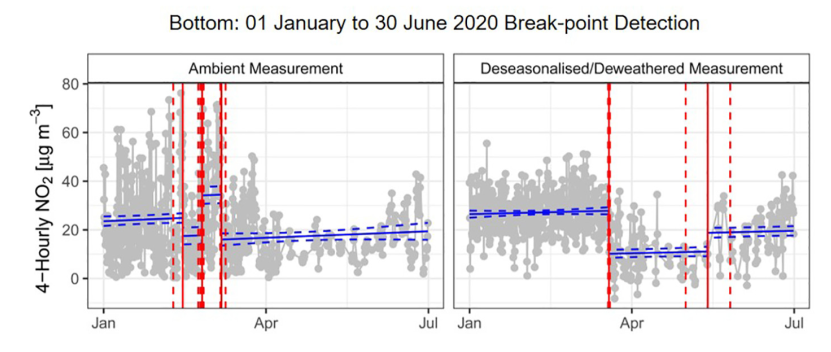
\includegraphics[width=1.\linewidth]{./figures/ropkins.png}
                                \end{figure}
                            \end{column}
                        \end{columns}
                    \item<3->{ \textbf{A.Briz-Redón et al.} }
                        \begin{columns}
                            \begin{column}{0.6\linewidth}
                                \tiny
                                \centering
                                \onslide<1->{
                                    \begin{equation*}
                                        \begin{align*}
                                            Pollutant_{i, t} =  & \alpha + \beta_1 temp_{i, t}
                                                + \beta_2 rain_{i, t} + \beta_3 wind_{i, t} \\
                                            & + \beta_4 sunlight_{i, t}
                                                + \beta_5 Maxpressure_{i, t} \\
                                            & + \gamma weekend_t + \rho_i city_i \\
                                            & + (\delta_1 + \delta_{1i}) minor_lockdown_t \\
                                            & + (\delta_2 + \delta_{2i}) major_lockdown_t \\
                                        \end{align*}
                                    \end{equation*}
                                }
                            \end{column}

                            \begin{column}{0.4\linewidth}
                                \begin{figure}[H]
                                    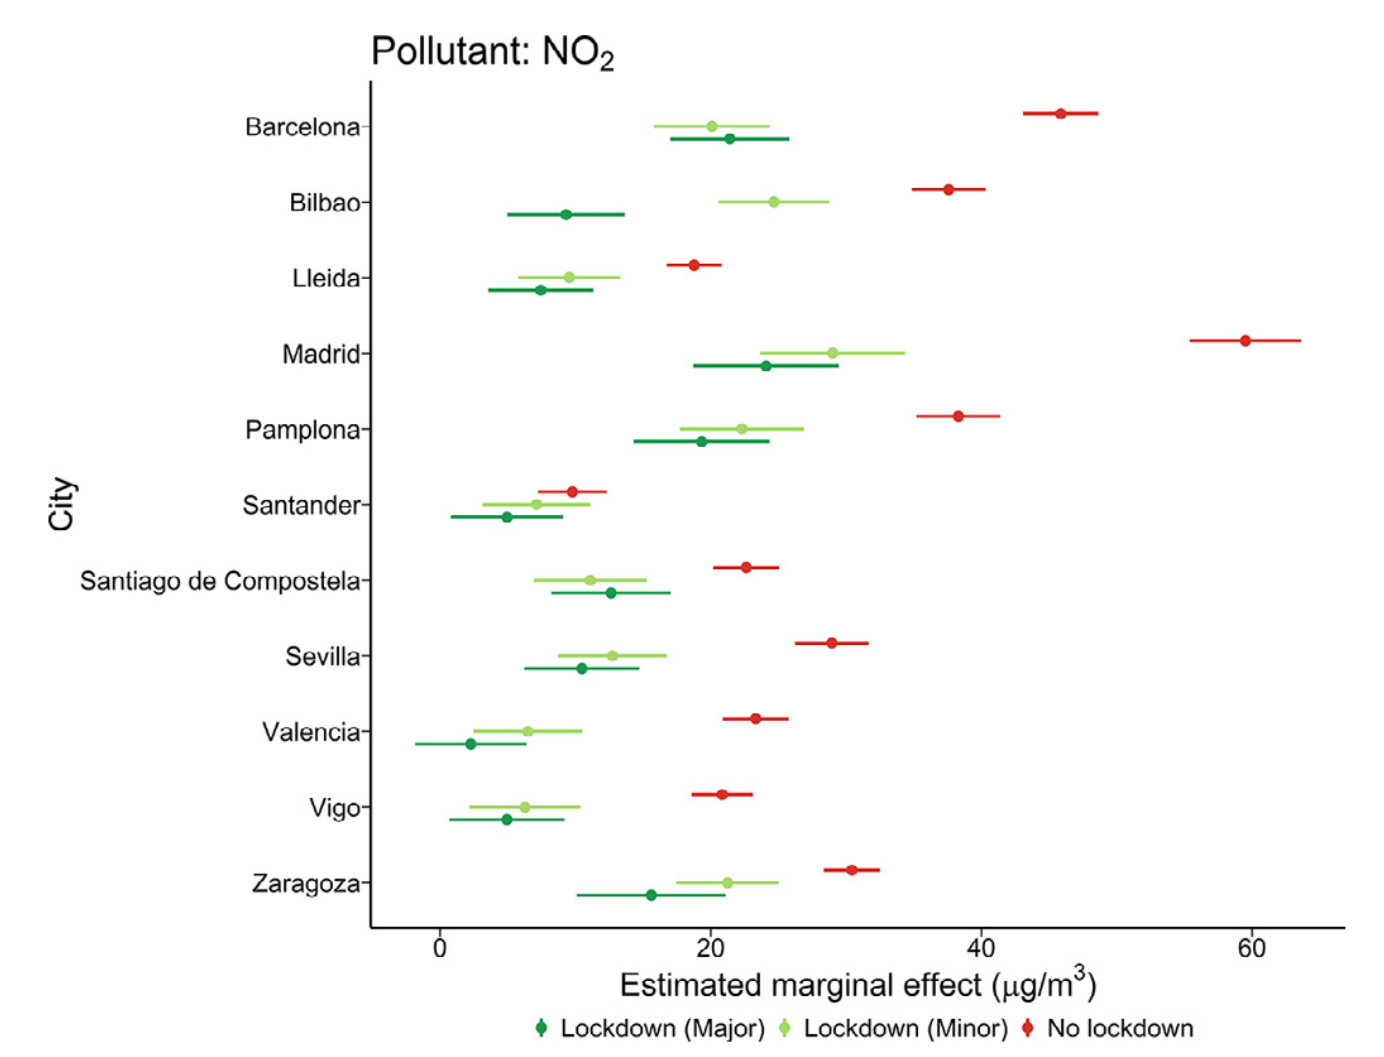
\includegraphics[width=.8\linewidth]{./figures/brizRedon.png}
                                \end{figure}
                            \end{column}
                        \end{columns}
                \end{itemize}
			\end{frame}

			\begin{frame}
				\frametitle{Analisis Claves}

                \begin{itemize}
                    \item<1->{Eliminar efectos estacionarios producidos por las distintas
                              estaciones del año}

                    \item<2->{Estudiar tendencias anuales de la calidad del aire en años anteriores}

                    \item<3->{Influencia de la meteorología en la calidad del aire}
                \end{itemize}
			\end{frame}
		\section{Nuestro estudio}

			\begin{frame}
				\frametitle{Elementos del Estudio}

                %\vspace{-2cm}
				\begin{itemize}
                    \item<1->{Datos de estaciones de tr\'afico urbano de ciudades españolas de m\'as de
                              100000 habitantes}
                    \vspace{0.5cm}
                    \item<2->{Contaminantes: $NO$, $NO_2$, $O_3$ y $PM_{10}$}
                    \vspace{0.5cm}
                    \item<3->{Datos del 2015-2020}
                \end{itemize}

                \vspace{1.5cm}
                \onslide<4->{ \begin{columns}
                    \tiny
                    \begin{column}{0.2\linewidth}
                        \centering
                        \onslide<1->{
                            Obtenci\'on de los datos mediante el paquete de \textbf{R}
                            \texttt{Openair} y \texttt{worldmet}
                        }
                    \end{column}

                    \begin{column}{0.05\linewidth}
                        \centering
                        \begin{equation*}
                            \Rightarrow
                        \end{equation*}
                    \end{column}

                    \begin{column}{0.2\linewidth}
                        \centering
                        Limpieza y tansformaci\'on de los datos
                    \end{column}
                    \begin{column}{0.05\linewidth}
                        \centering
                        \begin{equation*}
                            \Rightarrow
                        \end{equation*}
                    \end{column}

                    \begin{column}{0.2\linewidth}
                        \centering
                        Influencia de factores externos a la calidad del aire
                    \end{column}
                    \begin{column}{0.05\linewidth}
                        \begin{equation*}
                            \Rightarrow
                        \end{equation*}
                    \end{column}

                    \begin{column}{0.2\linewidth}
                        Cuantificaci\'on del efecto del confinamiento en la calidad del aire
                    \end{column}
            \end{columns}}
			\end{frame}


	%----------------------------------------------------------------------------
	%     BIBLIOGRAPHY
	%----------------------------------------------------------------------------

		\bibliographystyle{unsrt}
		\bibliography{biblio}

	\end{document}
